\documentclass[fleqn]{article}
\usepackage{amsmath, amssymb, esdiff}
\usepackage{gensymb}
\usepackage{tikz, pgfplots}
\usepackage{datetime}
\usepackage{ulem}
\usepackage{xcolor}
\usepackage{enumerate}
\setcounter{secnumdepth}{4}
\newcommand\numberthis{\addtocounter{equation}{1}\tag{\theequation}}


%opening
\title{Lecture 4}
\author{}
\date{\formatdate{6}{11}{2014}}

\begin{document}

\maketitle
\setlength{\mathindent}{0pt}

\tableofcontents

\newpage
\section{Vectors}

\subsection{Notation}

\begin{align*}	
	A &= \left| \overrightarrow{A} \right| = \left\| \overrightarrow{A} \right\| \\
	\hat{A} &\doteq \dfrac{\overrightarrow{A}}{A}\\
	\hat{z} &\doteq \hat{x} \times \hat{y}
	\hspace{1cm}
	\begin{tikzpicture}
		\draw [->](0,0) -- (0,1);
		\node [left] at (0,1) {$\hat{y}$};
		\draw [->](0,0) -- (1,0);
		\node [below] at (1,0) {$\hat{x}$};
		\draw [->](0,0) -- (-0.6,-0.4);
		\node [below] at (-0.6,-0.4) {$\hat{z}$};
	\end{tikzpicture}\\
	\overrightarrow{r} &= x \hat{x} + y \hat{y} + z \hat{z}\\
	r &= \sqrt{x^2 + y^2 + z^2}
\end{align*}

\subsection{Vector Addition}

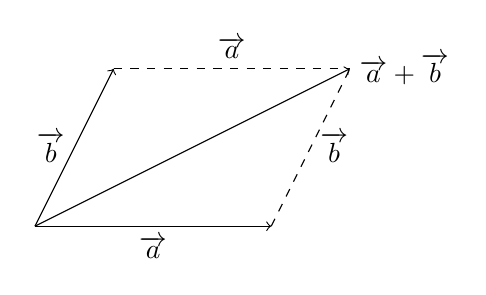
\begin{tikzpicture}
	\draw [->] (0,0) -- (3,0);
	\node [below] at (1.5,0) {$\overrightarrow{a}$};
	\draw [dashed] (3,0) -- (4,2);
	\node [above] at (2.5,2) {$\overrightarrow{a}$};
	\draw [->] (0,0) -- (1,2);
	\node [left] at (0.5,1) {$\overrightarrow{b}$};
	\draw [dashed] (1,2) -- (4,2);
	\node [right] at (3.5,1) {$\overrightarrow{b}$};
	\draw [->] (0,0) -- (4,2);
	\node [right] at (4,2) {$\overrightarrow{a} + \overrightarrow{b}$};
\end{tikzpicture}

\subsection{Scalar Product/ Dot Product}

\begin{tikzpicture}
	\draw [->] (0,0) -- (5,0);
	\node [right] at (5,0) {$\overrightarrow{a}$};
	\draw [->] (0,0) -- (3,2);
	\node [above] at (3,2) {$\overrightarrow{b}$};
	\node [above left] at (1,0) {$\theta$};
	\draw [dashed] (3,2) -- (3,0);
	\draw [red][->] (0,0) -- (3,0);
	\node [below] at (1.5,0) {$\overrightarrow{b} \cos \theta$};
\end{tikzpicture}

\begin{equation*}
	\overrightarrow{A} \cdot \overrightarrow{B} = A B \cos \theta
\end{equation*}

\subsubsection{Properties}

\begin{align*}
	\overrightarrow{A} \cdot \overrightarrow{B} &= \overrightarrow{B} \cdot \overrightarrow{A}\\
	\overrightarrow{A} \cdot (\overrightarrow{B} + \overrightarrow{C}) &= \overrightarrow{A} \cdot \overrightarrow{B} + \overrightarrow{A} \cdot \overrightarrow{C}
\end{align*}
If 
\begin{align*}
	r_1 &= (x_1 \hat{x} + y_1 \hat{y} + z_1 \hat{z})\\
	r_2 &= (x_2 \hat{x} + y_2 \hat{y} + z_2 \hat{z})
\end{align*}
\begin{align*}
	\overrightarrow{r_1} \cdot \overrightarrow{r_2} &= (x_1 \hat{x} + y_1 \hat{y} + z_1 \hat{z}) \cdot (x_2 \hat{x} + y_2 \hat{y} + z_2 \hat{z})\\
	&= x_1 x_2 + y_1 y_2 + z_1 z_2
\end{align*}

\subsubsection{Projection of Vectors}

The projection of $\overrightarrow{B}$ on $\overrightarrow{A}$ is denoted by $\overrightarrow{B}_{\overrightarrow{A}} $
\begin{align*}
	\overrightarrow{B}_{\overrightarrow{A}} &= \left(\dfrac{\overrightarrow{B} \cdot \overrightarrow{A}}{A}\right) \cdot \hat{A}\\
	&= \left(\dfrac{\overrightarrow{B} \cdot \overrightarrow{A}}{A}\right) \cdot \dfrac{\overrightarrow{A}}{A}\\ 
	&= \left(\dfrac{\overrightarrow{B} \cdot \overrightarrow{A}}{A^2}\right) \cdot \overrightarrow{A}
\end{align*}

\subsection{Vector Product/ Cross Product}

\begin{equation*}
	\overrightarrow{A} \times \overrightarrow{B} = A B \sin \theta \hat{r} ; \hat{r} \perp \overrightarrow{A}, \hat{r} \perp \overrightarrow{B}
\end{equation*}
\begin{equation*}
	\left\| \overrightarrow{A} \times \overrightarrow{B} \right\| = A B \sin \theta = \text{Area of parallelogram formed by $\overrightarrow{A}$ and $\overrightarrow{B}$} 
\end{equation*}

\subsubsection{Properties}

\begin{align*}
\overrightarrow{A} \times \overrightarrow{B} &= - \overrightarrow{B} \times \overrightarrow{A}\\
\overrightarrow{A} \times (\overrightarrow{B} + \overrightarrow{C}) &= \overrightarrow{A} \times \overrightarrow{B} + \overrightarrow{A} \times \overrightarrow{C}
\end{align*}

If 
\begin{align*}
	r_1 &= (x_1 \hat{x} + y_1 \hat{y} + z_1 \hat{z})\\
	r_2 &= (x_2 \hat{x} + y_2 \hat{y} + z_2 \hat{z})
\end{align*}
\begin{align*}
	\overrightarrow{r_1} \times \overrightarrow{r_2} &= (x_1 \hat{x} + y_1 \hat{y} + z_1 \hat{z}) \times (x_2 \hat{x} + y_2 \hat{y} + z_2 \hat{z})\\
	&= 
	\begin{vmatrix}
		\hat{x} & \hat{y} & \hat{z}\\
		x_1 & y_1 & z_1\\
		x_2 & y_2 & z_2\\
	\end{vmatrix}
\end{align*}

\section{Derivatives of Vectors}

\begin{align*}
	\overrightarrow{v} &= \diff{\overrightarrow{r}}{t}\\
	&= \lim\limits_{\Delta t \rightarrow 0} \dfrac{\overrightarrow{r}(t + \Delta t) - \overrightarrow{r}(t)}{\Delta t}\\
	\overrightarrow{a} &= \diff{\overrightarrow{v}}{t} = \dot{\overrightarrow{v}} = \ddot{\overrightarrow{r}}
\end{align*}

\subsection{Properties}

\begin{equation*}
	\diff{}{t} (\overrightarrow{A} \times \overrightarrow{B}) = \diff{\overrightarrow{A}}{t} \times \overrightarrow{B} + \overrightarrow{A} \times \diff{\overrightarrow{B}}{t}
\end{equation*}

\end{document}